\documentclass[12pt,a4]{article}
\usepackage[left=1.8cm,right=1.8cm,top=32mm,columnsep=20pt]{geometry}

\usepackage[utf8]{inputenc} %Formato de codificación
\usepackage[spanish, es-tabla, es-nodecimaldot]{babel}
\usepackage{amsmath} %paquete para escribir ecuaciones matemáticas
\usepackage{float} %Para posicionar figuras
\usepackage{graphicx} %Para poder poner figuras
\usepackage{tikz}
\usepackage{subcaption}
\usetikzlibrary{positioning}
\usetikzlibrary{shapes.geometric, decorations.pathreplacing}

\title{Analisis movimiento de un pendulo}
\author{Francisco Carruthers, Facundo Firpo y Joel Jablonski\\ [2mm]
\small \texttt{\{fcarruthers, ffirpo, jjablonski\}@udesa.edu.ar}\\
\small Fisica I, tutorial Vinograd}
\date{2do Semestre 2024}


\begin{document}

\maketitle

\begin{abstract}
    Se investigó el movimiento de un péndulo simple variando la longitud de la cuerda, la masa del péndulo y el angulo inicial. 
    El objetivo principal fue registrar y caracterizar su trayectoria, determinar el rango angular donde se cumplen las condiciones de pequeñas oscilaciones, calcular la frecuencia de oscilación y estimar la gravedad efectiva. 
    Primero, se mantuvo una longitud fija de cuerda, variando los ángulos iniciales con diferentes masas, y luego se analizó cómo la longitud de la cuerda afecta el movimiento al fijar el ángulo y la masa. 
    La gravedad efectiva obtenida fue de $(9.5 \pm 0.6) \text{m/s}^2$ que tiene sentido ya que incluye a la gravedad real. 
    Además, evaluamos la influencia de los parámetros sobre la frecuencia de oscilación ($\omega$) del péndulo, concluyendo que, aunque la masa no altera la frecuencia, la longitud sí lo hace con una relacion cuadratica. 
    Finalmente, se identificó el rango de ángulos donde se cumplen pequeñas oscilaciones, siendo de aproximadamente ángulos menores a $30^\circ$.

\end{abstract}

\section{Introducción}

El estudio del péndulo simple ha sido fundamental en la comprensión de la dinámica oscilatoria y los principios físicos básicos que la rigen. 
Este informe se centra en analizar cómo variables clave como el ángulo inicial, la longitud de la cuerda y la masa del péndulo afectan su periodo de oscilación y frecuencia angular. 
Además, se evalúa la validez del régimen de pequeñas oscilaciones, caracterizando la dependencia de los parámetros del sistema con el comportamiento observado. 
Este trabajo tiene como objetivo proporcionar una comprensión de estos principios fundamentales.

\section{Marco teorico}

El pendulo se modela de la siguiente forma:

\begin{figure}[H]
    \centering
    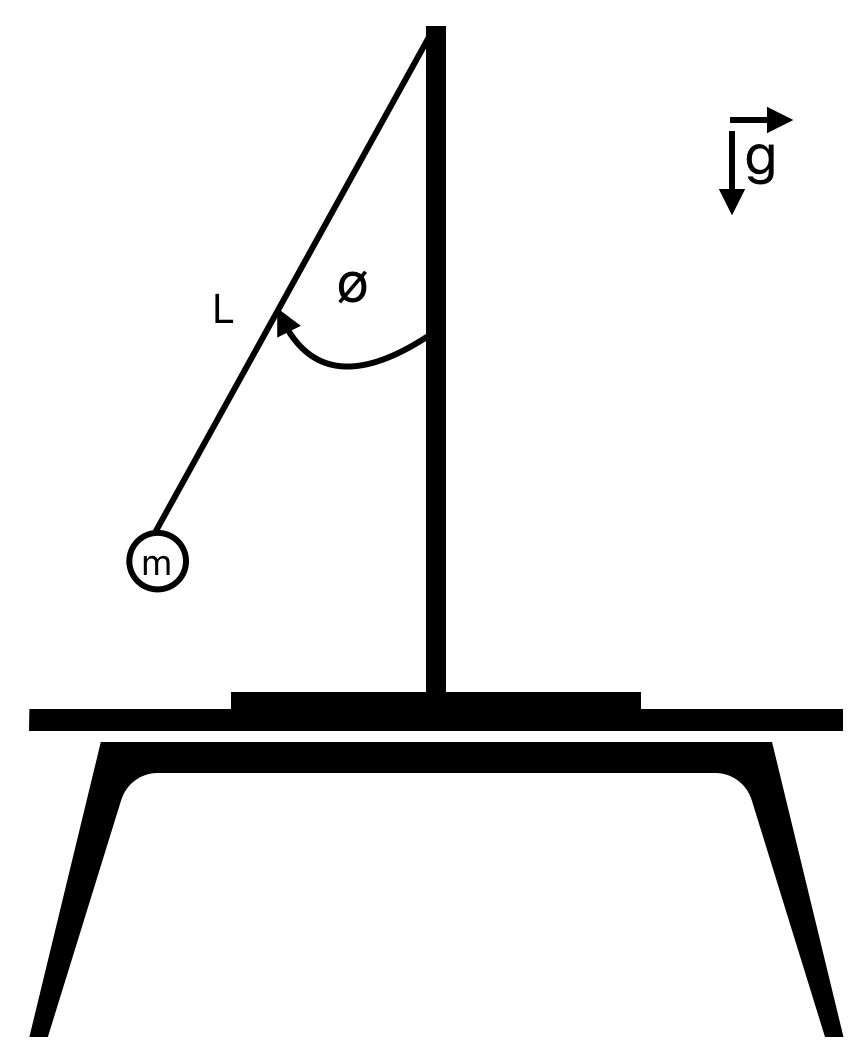
\includegraphics[width=0.3\linewidth]{pendulo_frente.png}
    \caption{Péndulo simple con longitud de soga L , masa m y ángulo de desplazamiento $\phi$}   
    \label{fig:pendulo}
\end{figure}

Para nuestro sistema, de las ecuaciones de Newton, obtenemos la ecuación diferencial que describe el movimiento del péndulo simple:

\begin{equation}
    \ddot{\phi} = -\frac{g}{L} \cdot sin(\phi)
\end{equation}

Donde $\phi$ es el ángulo de desplazamiento, $g$ es la aceleración debida a la gravedad y $L$ es la longitud de la cuerda. 
Para pequeñas oscilaciones, podemos aproximar $sin(\phi) \approx \phi$ y obtener la solución general de la ecuación diferencial:

\begin{equation}
    \phi(t) = A \cdot cos(\omega t + \varphi)
\end{equation}

Donde $A$ y $\varphi$ son determinados por las condiciones iniciales. 
En nuestro caso, $\dot{\phi}(t=0) = 0$ y $\phi(t=0) = \phi_0$. 
Por otro lado, $\omega$ , la frecuencia de un péndulo simple, esta dada por:

\begin{equation}
    \omega = \sqrt{\frac{g}{L}}
    \label{eq:omega}
\end{equation}

\begin{equation}
    T = 2 \pi \frac{1}{\omega}
    \label{eq:periodo}
\end{equation}

Esta ecuación asume que el péndulo oscila en el régimen de pequeñas oscilaciones. 
Donde podemos definir que $sin(\phi) \approx \phi$ para ángulos pequeños. 
En la practica intentamos verificar esta aproximación y encontrar hasta que $\phi$ se cumple al variar los ángulos iniciales y comparando el movimiento con el esperado.

La ecuación \ref{eq:omega} indica que este es independiente tanto de la masa del péndulo como de su ángulo inicial en el régimen de pequeñas oscilaciones, pero depende de la longitud de la cuerda. 
Esto sugiere que, al reducir la longitud de la cuerda, la frecuencia angular aumentará, reflejando un ciclo de oscilación más rápido.

\section{Práctica experimental}

Para poder estudiar el movimiento de la masa en el péndulo simple, se realizó un experimento en el cual se variaron los parámetros del sistema, como la longitud de la soga, la masa de la bolita y el ángulo inicial.
Se filmaron los movimientos de la masa y se analizaron los videos para obtener datos sobre la posición de la masa en función del tiempo.
El pendulo se armo como el visto en la Figura \ref{fig:pendulo} al cual se le coloco una camara de X fps con X resolucion para poder seguir el movimiento de la masa.

COMPLETAR FPSSSS y RESOLUCION

\begin{figure}[H]
    \centering
    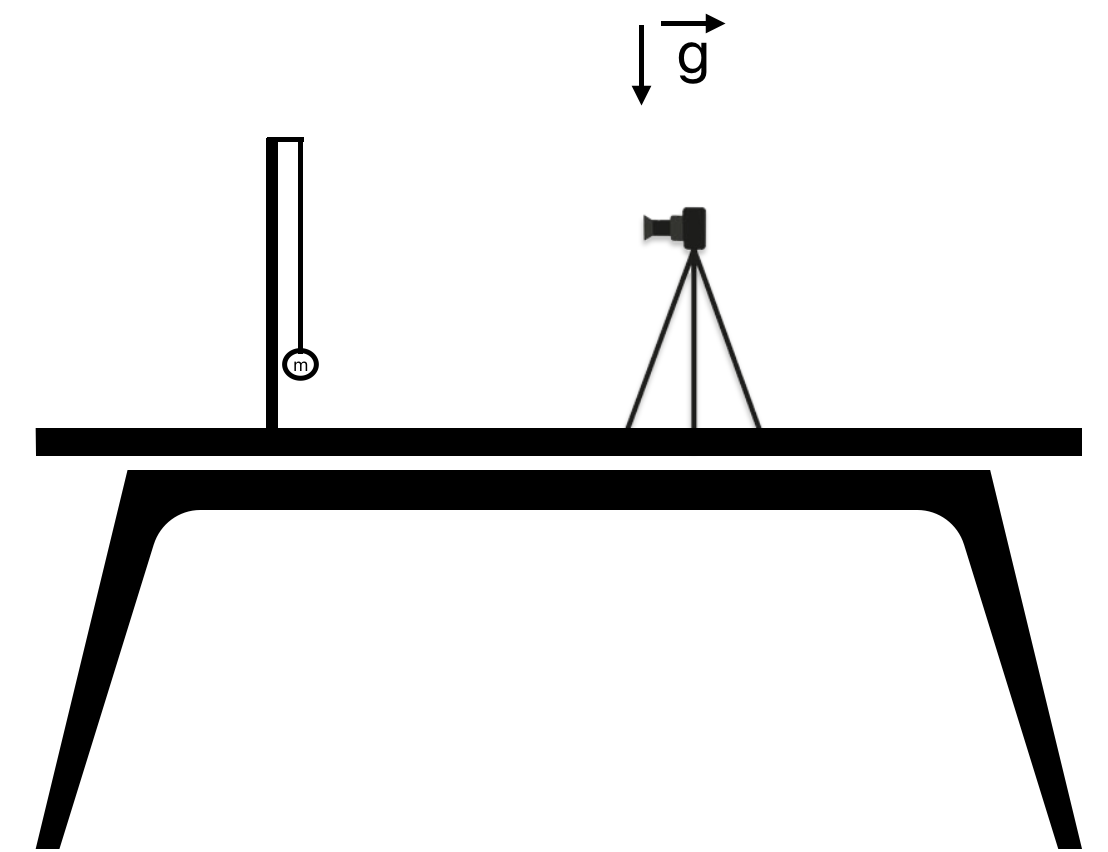
\includegraphics[width=0.6\linewidth]{esquema.png}
    \caption{Esquema del experimento}   
    \label{fig:esquema}
\end{figure}

La masa y la longitud de la soga se pueden variar, lo que nos permitió experimentar con diferentes condiciones iniciales y observar sus efectos en el comportamiento del péndulo simple.

Para la obtención de datos, utilizamos un teléfono para filmar los movimientos del péndulo y posteriormente analizamos los videos con el programa \textit{Tracker}, que permite seguir una masa específica en función del tiempo y registrar su posición. 
Para obtener una referencia de distancia, colocamos una cinta métrica en el fondo de cada video, permitiendo al programa calibrar la relación entre píxeles y distancia real y, así, establecer la posición de la masa con precisión.

Una vez construido el sistema, procedimos con el experimento. Hicimos 9 mediciones en total, variando la longitud de la soga, la masa de la bolita y el ángulo inicial.

Primero, para estudiar la dependencia de la frecuencia de oscilación con respecto a la longitud de la soga, mantuvimos una masa constante de $(23 \pm 1) \, \text{g}$ y un ángulo inicial de $(25 \pm 2)^\circ$ y variamos la longitud de la soga con valores entre 
42 y 15 cm donde el error de los largos esta dado por la medicion minima de la cinta metrica usada siendo esta de $\pm 0.1 cm$.

Luego, para estudiar la dependencia de la frecuencia de oscilación con respecto a la masa, mantuvimos una longitud fija de $(42.0 \pm 0.1) \, \text{cm}$ y un ángulo inicial de $(25 \pm 2)^\circ$ y variamos la masa con valores entre 
5 y 72 g donde el error asociado a las masas se define por la unidad minima mostrada por la balanza usada siendo esta de $\pm 1 g$.

Para estudiar la dependencia de la frecuencia de oscilación con respecto al ángulo inicial, mantuvimos una longitud fija de $(42.0 \pm 0.1) \, \text{cm}$ y una masa de $(23 \pm 1) \, \text{g}$ y variamos los ángulos iniciales con valores entre 
$55^\circ$ y $10^\circ$ donde el error de cada angulo se consigue con la formula de propagacion de errores. 
Teniendo en cuenta que usamos: $sin(\phi) = \frac{opuesto}{hipotenusa}$ para definir el $\phi_0$, entonces el error de $\phi$ se calcula como:

\begin{equation}
    \Delta \phi = \sqrt{\left( \frac{\partial \phi}{\partial (\text{opuesto})} \Delta (\text{opuesto}) \right)^2 + \left( \frac{\partial \phi}{\partial (\text{hipotenusa})} \Delta (\text{hipotenusa}) \right)^2}
\end{equation}

Donde $\Delta (\text{opuesto}) = 1 cm$ por nuestro error al medir la distancia entre la posicion inicial de la masa y la barra del pendulo,
 y $\Delta (\text{hipotenusa}) = 0.1 cm$.

Para seguir la trayectoria descargamos los videos de los experimentos y los abrimos en el programa \textit{Tracker}. 
Luego, seleccionamos la masa y seguimos su trayectoria en función del tiempo usando un feature que ofrece la aplicación. 
También, definimos un sistema de coordenadas polares con el origen en el inicio de la soga. 
Para determinar distancias en el video, colocamos una cinta métrica en el fondo de la escena y calibramos el programa para que pueda determinar distancias en el video. 
El seguimiento de la masa en el programa no es perfecto, por lo que se observan errores en la trayectoria obtenida.
El programa al seguir a la masa, no siempre esta centrado en el centro de la masa por lo que a la posicion de la masa se le debe agregar un error adicional de 1 cm (el radio de la masa) tanto verticalmente como horizontalmente.

A partir de las mediciones obtenidas, buscamos estimar una gravedad efectiva mediante el análisis de la pendiente en la gráfica de \( T^2 \) frente a la longitud \( L \) que se puede obtener de la ecuacion \ref{eq:periodo}, considerando que esta pendiente corresponde a:
\begin{equation}
    T^2 = \frac{4 \pi^2}{g} L
    \label{eq:gravedad}
\end{equation}

Este enfoque permite no solo una estimación experimental de \( g \), sino también la evaluación de la precisión de nuestro sistema. 

\section{Resultados}

\begin{figure}[H]
    \centering
    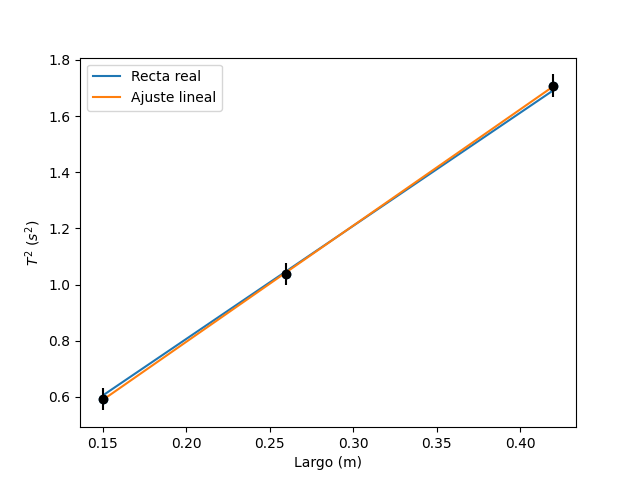
\includegraphics[width=0.6\linewidth]{gravedad.png}
    \caption{Regresión lineal de \( T^2 \) vs \( L \) para estimar la gravedad usando $m = (23 \pm 1) \, \text{g}$ y $\phi = (25 \pm 1)^\circ$}
    \label{fig:gravedad}
\end{figure}

Despejando g de la pendiente dada en la ecuacion \ref{eq:gravedad} la recta obtenemos: $g = 9.5 \pm 0.6 m/s^2$. Este parámetro incluye a la gravedad real y a los errores de medición del experimento. Se puede observar que el valor obtenido es consistente con el valor teórico esperado de $9.8 m/s^2$ en la recta azul que tiene una pendiente de $\frac{4\pi^2}{9.8}$.

A continuación, analizamos la relación entre el periodo de oscilación y la longitud de la soga. Dejando fijos la masa ($23 \pm 1) g$ y el angulo inicial ($25 \pm 1) ^\circ$ obteniendo los siguientes resultados:

\begin{figure}[H]
    \centering
    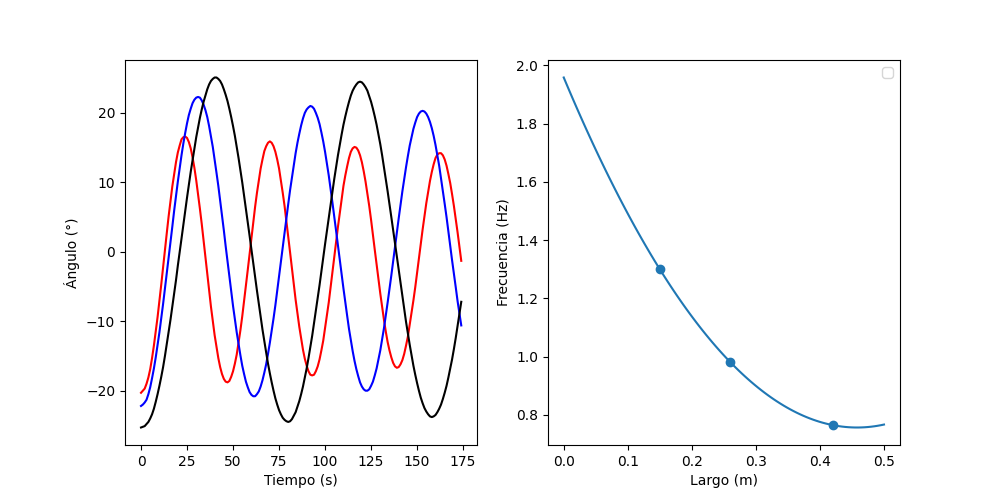
\includegraphics[width=0.6\linewidth]{largo.png}
    \caption{Posición de la masa en función del tiempo, y frecuencia de oscilación para distintos largos de soga con valores constantes m = ($23 \pm 1) g$ y ($25 \pm 1) ^\circ$.}
    \label{fig:largo}
\end{figure}

Se puede observar como el largo de la soga afecta la frecuencia del movimiento. A mayor largo, menor frecuencia. Esto se debe a que la bolita recorre una mayor distancia. Sabemos que la longitud de arco esta definida como $d = r \phi$, donde $d$ es la longitud de arco, que es la distancia que recorre la bolita a lo largo de su trayectoria circular, y $r$ es el radio del círculo, que en este caso es la longitud de la soga hasta la bolita; por lo que a mayor longitud de soga, mayor longitud de arco recorre la bolita.

\begin{figure}[H]
    \centering
    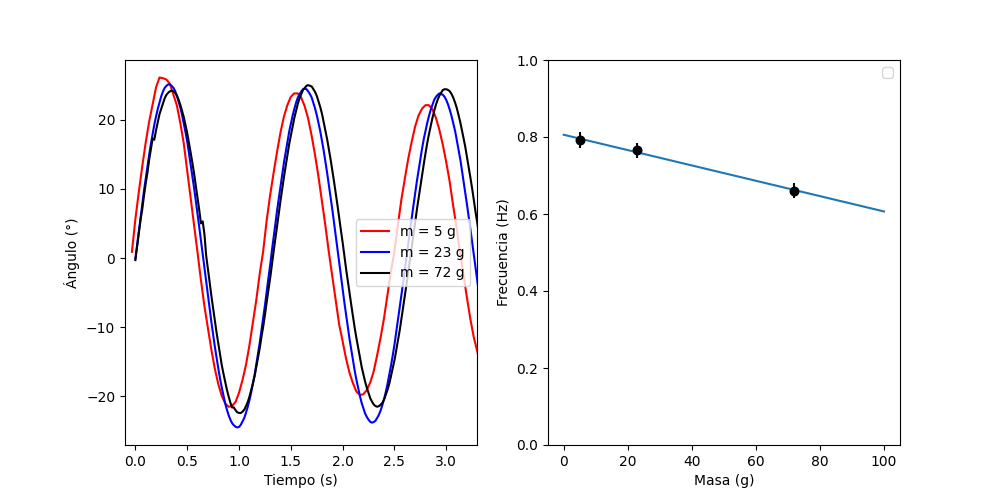
\includegraphics[width=0.6\linewidth]{peso.png}
    \caption{Posición de la masa en función del tiempo, y frecuencia de oscilación en función del largo para distintas masas con valores constantes L = $(42.0 \pm 0.1)$ cm y $\phi$ = $(25 \pm 1) ^\circ$.}
    \label{fig:masa}
\end{figure}

En la Figura \ref{fig:masa} se observa cómo la frecuencia del movimiento parece depender de la masa de la bolita. Sin embargo, teóricamente, para pequeñas oscilaciones en un péndulo simple ideal, la frecuencia no debería depender de la masa, ya que viene determinada únicamente por la longitud de la soga y la gravedad.

La tendencia observada en el experimento puede deberse a que la soga no es perfectamente rígida, lo que introduce una dependencia con la masa debido a deformaciones o tensiones adicionales. Esto podría explicar la desviación de la teoría ideal en los resultados experimentales.

Luego, variamos los ángulos iniciales dejando fijo la masa en ($23 \pm 1) g$ y largo de la soga en ($42.0 \pm 0.1) cm$ para poder analizar la suposición de pequeñas oscilaciones. Para los distintos ángulos iniciales se obtuvieron los siguientes resultados:

\begin{figure}[H]
    \centering
    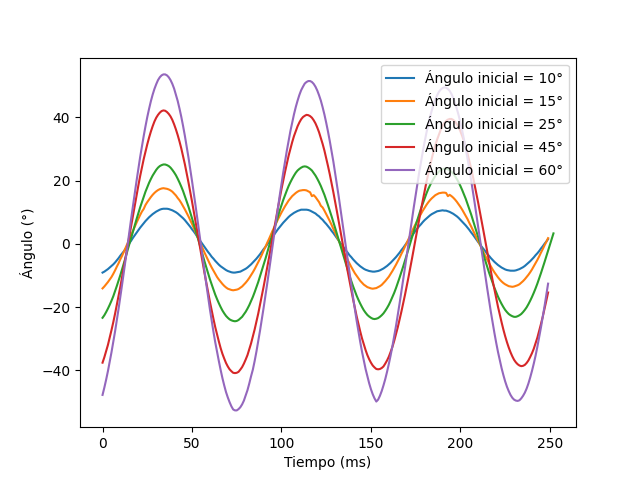
\includegraphics[width=0.6\linewidth]{angulos.png}
    \caption{Posición de la masa en función del tiempo y frecuencia de oscilación para distintos ángulos iniciales con valores constantes m = ($23 \pm 1) g$ y L = $(42.0\pm0.1)$ cm.}
    \label{fig:angulos}
\end{figure}

Se puede observar como la amplitud del movimiento no afecta la frecuencia del mismo. El gráfico \ref{fig:angulos} muestra como la relación entre la frecuencia y el largo de la soga se mantiene prácticamente constante, con una pequeña pendiente debido al error de medición, para distintos ángulos iniciales. Esto coincide con la suposición de pequeñas oscilaciones.

Para determinar el rango de ángulos en el cual se cumple la aproximación de pequeñas oscilaciones en el péndulo, calculamos el error cuadrático medio (ECM) entre las trayectorias experimentales medidas y las trayectorias obtenidas mediante la aproximación lineal. 

\[
\text{ECM} = \frac{1}{n} \sum_{i=1}^{n} (y_i - \hat{y}_i)^2
\]

Donde $y_i$ es la posición de la masa en el tiempo $i$ medida experimentalmente y $\hat{y}_i$ es la posición de la masa en el tiempo $i$ calculada mediante la aproximación de pequeñas oscilaciones.
\begin{figure}[H]
    \centering
    \begin{minipage}{0.5\textwidth}
        \centering
        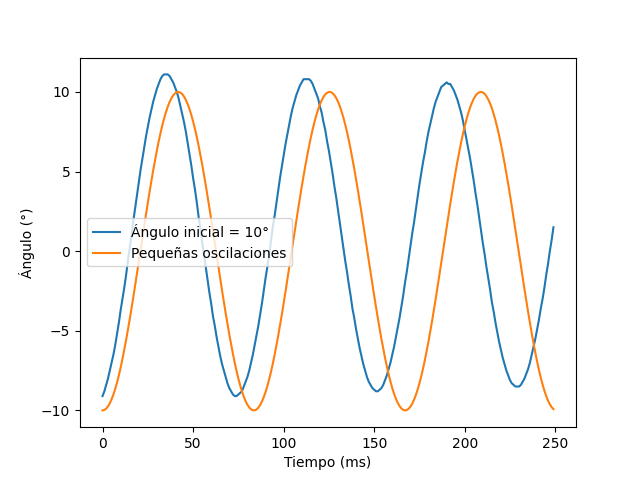
\includegraphics[width=\textwidth]{peq_osc_10.png}
    \end{minipage}%
    \begin{minipage}{0.5\textwidth}
        \centering
        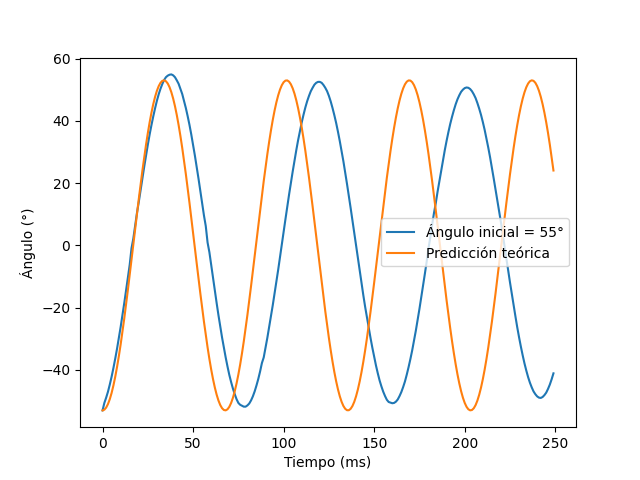
\includegraphics[width=\textwidth]{peq_osc_55.png}
    \end{minipage}
    \caption{Comparacion entre datos obtenidos y su prediccion teorica correspondiente para angulos iniciales de $10^\circ$ y $55^\circ$.}
    \label{fig:comparacion_angulos}
\end{figure}

En la Figura \ref{fig:comparacion_angulos} se puede observar que para el ángulo de $10^\circ$ la aproximación de pequeñas oscilaciones es válida, mientras que para el ángulo de $55^\circ$ la aproximación no lo es, ya que no aproxima lo suficientemente bien a la prediccion teorica.

El valor del ECM se presenta en la Figura \ref{fig:pequeñas_oscilaciones}, donde se observa cómo varía con el ángulo inicial.

\begin{figure}[H]
    \centering
    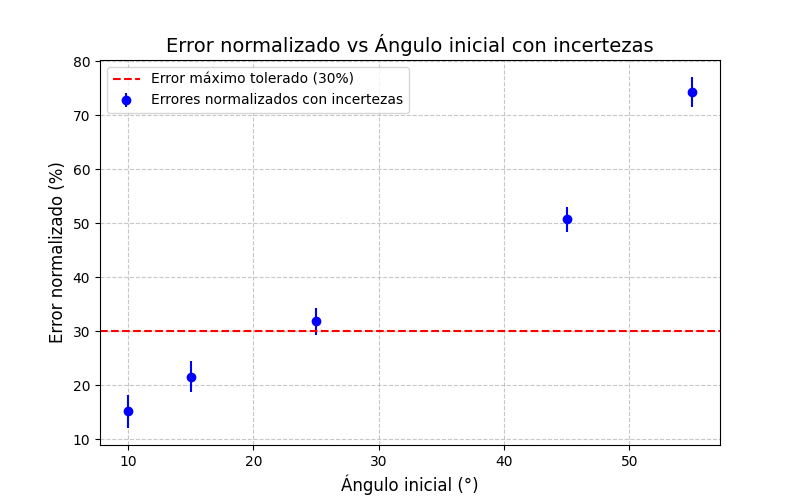
\includegraphics[width=0.6\linewidth]{errores_normalizados_incertezas.png}
    \caption{Error cuadrático medio bajo la aproximación de pequeñas oscilaciones con m = $(23\pm1)$ g y L = $(42.0\pm0.1)$ cm.}
    \label{fig:pequeñas_oscilaciones}
\end{figure}
Observando el gráfico de la Figura \ref{fig:pequeñas_oscilaciones}, determinamos que la aproximación de pequeñas oscilaciones es válida hasta aproximadamente \(25^\circ\). Para identificar el ángulo máximo que cumple esta condición, calculamos el error cuadrático medio normalizado respecto al ángulo inicial, considerando las incertidumbres asociadas. Decidimos tolerar un error máximo del \(30\%\). Como se observa en el gráfico, el error correspondiente a \(25^\circ\) es el ángulo máximo que, considerando sus incertidumbres, cumple con nuestra tolerancia.

Este resultado sugiere que, para ángulos iniciales menores a \(25^\circ\), la trayectoria experimental se ajusta adecuadamente a la predicha por la teoría de pequeñas oscilaciones, cumpliendo así con las condiciones lineales esperadas.

\section{Conclusiones}

Se investigó el comportamiento de un péndulo simple y su relación con la longitud de la cuerda y la masa del péndulo, confirmando que bajo la asumpción de pequeñas oscilaciones la frecuencia de oscilación depende únicamente de la longitud. La gravedad efectiva obtenida fue de \((9.5 \pm 0.6) \, \text{m/s}^2\), consistente con el valor teórico esperado el cual es \(9.8 \, \text{m/s}^2\). Se observaron frecuencias angulares (\(\omega\)) de \((0.75 \pm 0.02)\, \text{s}^{-1}\) para \(42 \, \text{cm}\), \((0.98 \pm 0.02) \, \text{s}^{-1}\) para \(26 \, \text{cm}\) y \((1.3 \pm 0.02) \, \text{s}^{-1}\) para \(15 \, \text{cm}\), corroborando la relación inversa entre longitud y frecuencia con los valores teóricos los cuales son \(0.77 \text{s}^{-1}\) para \(42 \, \text{cm}\), \(0.98 \text{s}^{-1}\) para \(26 \, \text{cm}\), \(1.29 \text{s}^{-1}\) para \(15 \, \text{cm}\), observamos que nuestros resultados son acertados de nuestro rango de error. Adicionalmente, se determinó que el rango de ángulos donde se cumplen las condiciones de pequeñas oscilaciones es aproximadamente hasta $25^\circ$. Estos resultados reafirman los principios de la dinámica oscilatoria y respaldan la aplicación del modelo de pequeñas oscilaciones en el estudio de sistemas físicos similares.

\end{document}